\documentclass[12pts]{report}


\usepackage{amssymb}
\usepackage{amsmath}
\usepackage{amscd}
\usepackage{amsthm}
\usepackage[utf8]{inputenc}
\usepackage[spanish,mexico]{babel}
\usepackage{enumerate}
\usepackage[usenames]{color}


\usepackage{pgf,tikz}
\usetikzlibrary{arrows}

\usepackage[colorlinks=true, linkcolor=blue, urlcolor=red,
citecolor=green]{hyperref}

\voffset=-2cm
\hoffset=-2cm
\textwidth = 18cm
\textheight= 23 cm

\usepackage{iwona}
\usepackage{fancyhdr}
\pagestyle{fancy}
\fancyhf{}
\fancyhead[RE,LO]{\bfseries{Seminario de Topologia B}}
\fancyhead[LE,RO]{\bfseries{2019-2}}
\fancyfoot[RE,RO]{\bfseries{febrero 2019}}
\fancyfoot[LE,LO]{\bfseries{Tarea 01}}

\newcommand{\R}{\mathbb R}
\newcommand{\Q}{\mathbb Q}
\newcommand{\E}{\mathbb E}
\newcommand{\s}{\mathbb S}
\newcommand{\C}{\mathbb C}
\newcommand{\F}{\mathbb F}
\newcommand{\T}{\mathbb T}
\newcommand{\p}{\mathbb P}
\newcommand{\I}{\mathbb I}
\newcommand{\A}{\mathbb A}
\newcommand{\h}{\mathbb H}

\begin{document}
\begin{center}
\textcolor{blue}{\textbf{\large Guia de ejercicios para la evaluación del primer parcial}}
\end{center}

\begin{enumerate}
\item Demostrar que las proyecciones regulares son densas en el conjunto de las proyecciones regulares.
\item Dibujar el nudo $T_{4,5}$.
\item Dibujar el nudo $C(3,8)$.
\item Sea $K$ un nudo. Si $K$ es dócil entonces existe una proyección regular de $K$.
\item Dibujar el nudo racional $l(2,-7)$.
\item Demostrar que la 5 coloración es un invariante en el conjunto de diagramas.
\item Dibujar un nudo satelital  usando el nudo  ocho y que tenga como corazón un nudo $T_{3, 5}$.
\item Encontrar un nudo que no sea $3$-coloreable ni $5$-coloreable.
\item Determinar los movimientos de Reidemeister para ver si se pueden desenredar los siguientes nudos y en caso de que no, determinar que nudo conocido es.
\begin{center}

\includegraphics[width=0.3\textwidth] {trebol.png}\quad
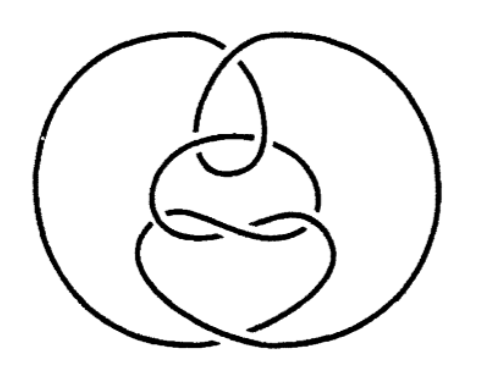
\includegraphics[width=0.3\textwidth]{desenredar.png}
\end{center}
\item Determinar que p-coloración tienen los siguientes nudos.
\begin{center}
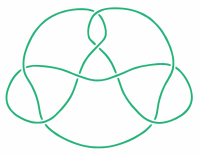
\includegraphics[width=0.3\textwidth] {diagrama1.png}\quad 
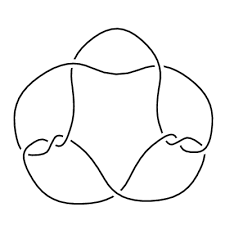
\includegraphics[width=0.3\textwidth] {diagrama2.png}
\end{center}
\end{enumerate}
\end{document}